Im Master könnt ihr euren Stundenplan relativ frei zusammenstellen. Wichtig ist dabei nur, dass du alle Wahlpflichtbereiche entsprechend deiner Prüfungsordnung abdeckst, also die geforderte Anzahl an Leistungspunkten\footnote{an verschiedenen Stellen auch als ECTS-Punkte oder Credit Points bezeichnet} in jedem Wahlpflichtfach mit Veranstaltungen füllst. Eine Auflistung aller Veranstaltungen und eine Zuordnung zu welchem Wahlpflichtbereich sie gehören, findest du in deinem Modulhandbuch. Eine Übersicht über alle Modulhandbücher findest du auf den Seiten des Fachbereichs Informatik: \\ 
\url{http://uni-tuebingen.de/de/74348}
%\fett{Überfachliche Berufsfeldorientierte Kompetenzen}
%Einen speziellen Bereich stellen hierbei noch die sogenannten übK (früher Schlüsselqualifikationen, SQ) dar. Dieser Wahlpflichtbereich ist dazu gedacht dich auch außerhalb deiner akademischen Disziplin weiterzubilden. Im Gegensatz zu vielen anderen Studiengängen an der Universität ist des dir erlaubt in diesem Bereich alle fachfremden Veranstaltungen (außer Sport) zu hören, solange sie benotet sind

\ifkogwiss
Für den Master Kognitionswissenschaft könnt ihr euch an dem abgebildeten Beispielstudienplan orientieren.
\begin{center}
	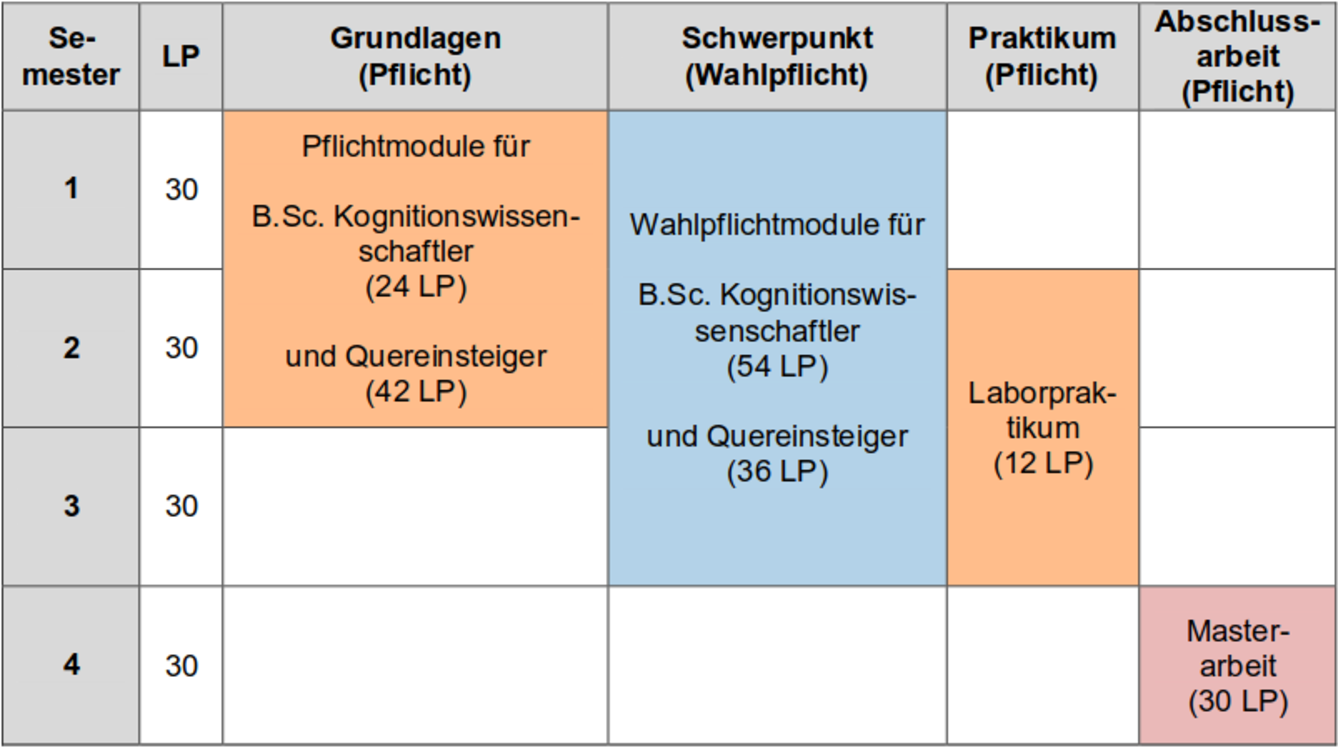
\includegraphics[width=.8\textwidth]{media/studienplan_kmsc.pdf}
\end{center}
%Genauere Informationen zu den einzelnen Modulen findet ihr im Modulhandbuch\\ (http://www.wsi.uni-tuebingen.de/studium/downloads/modulhandbuecher.html). \\
%\\
Zu beachten ist die Gewichtung der verschiedenen Module und die Reihenfolge, in der die Module mit Kursen aufgefüllt werden. Wenn
ihr z.B. das Modul MKOGINF mit Informatikkursen aufgefüllt habt, ist es unter Umständen schwierig, diese Kurse durch Kurse mit
besserer Note zu ersetzen. Nähere Informationen dazu werden euch bei der Einführungsveranstaltung zum Master Kognitionswissenschaft mitgeteilt. Ferner spielen im Master für einige Studierende Auflagen eine wichtige Rolle. In eurem Zulassungsbescheid seid ihr darüber informiert worden, ob ihr in der Psychologie und/oder Informatik Auflagen erfüllen müsst. Dies bedeutet, dass ihr in dem jeweiligen Fach einige Grundveranstaltungen besuchen müsst. Zu den Auflagen bekommt ihr ebenfalls bei der Einführungsveranstaltung genauere Informationen mitgeteilt. In seltenen Fällen können Auflagen gestrichen werden, falls im Bachelor vergleichbare Leistungen erbracht wurden. Hierfür könnt ihr euch an Frau Seibold wenden, die die Angelegenheit mit dem Studiendekan Prof. Wichmann abklärt (anerkennung\At kogwis.uni-tuebingen.de). Generell könnt ihr euch bei Fragen zur Studienorganisation ebenso bei Frau Seibold melden (studienberatung\At kogwis.uni-tuebingen.de). Exemplarische Studienpläne, abhängig von euren Auflagen, könnt ihr auch im Modulhandbuch nachsehen, welches ihr hier findet: https://www.wsi.uni-tuebingen.de/studium/downloads/modulhandbuecher-und-veranstaltungsverzeichnisse.html.

\fi

\ifinfo
Manche Veranstaltungen können, abhängig vom Studiengang, in verschiedenen Bereichen angerechnet werden, z.B. können im Master-Studium Informatik viele Veranstaltungen der praktischen Informatik sowohl im Bereich \textbf{INFO-PRAK} als auch im Bereich \textbf{INFO-INFO} angerechnet werden. Wichtig ist hierbei, dass eine Veranstaltung logischerweise nur in \emph{einem} Bereich angerechnet werden kann. Unsere Empfehlung: Führe selbst Buch darüber, welche Veranstaltung du in welchem Bereich einbringen willst. \\\\
\iflehramt
Für die Wahlpflichtbereiche des \textbf{Master of Education} solltest du einen Blick ins Modulhandbuch werfen. Dieses findest du unter \url{https://uni-tuebingen.de/de/111771}.
\else
\fett{Schwerpunkt}
Des weiteren musst du dir im Masterstudiengang Informatik ein Schwerpunktfach wählen. Das Schwerpunktfach setzt sich aus 18 LP, welche normalerweise in verschiedenen Veranstaltungen eines anderen Fachbereichs erreicht werden müssen, zusammen. Es ist jedoch auch möglich, diesen Bereich komplett mit Informatik-Veranstaltungen zu füllen. Näheres hierzu findest du auch im Modulhandbuch. 
\fi
\fi\
